% Cover letter: Platform Product Designer, Revolut
% CV: Sections/cv_product_designer.tex -> cv_gen/cv_giovanni_tauro-revolut.pdf
\documentclass[11pt,a4paper,sans]{moderncv}
% Shared preamble and header for the cover letters.
% One main file per application: cl_<company>.tex, built to
% cv_gen/coverletter_giovanni_tauro-<company>.pdf next to cv_giovanni_tauro-<company>.pdf.
% Paths (cl_gen/..., Pictures/...) are relative to the project root, as in the CV (see .latexmkrc).

\moderncvstyle{classic}
\moderncvcolor{blue}

\usepackage[scale=0.80]{geometry}
\setlength{\footskip}{136.00005pt}

\usepackage{fontawesome5}
% hyperref is loaded by moderncv itself; loading it here causes an option clash
\usepackage{xcolor}
\usepackage{graphicx}
\ifxetexorluatex
  \usepackage{fontspec}
  \usepackage{unicode-math}
  \defaultfontfeatures{Ligatures=TeX}
  \setmainfont{Latin Modern Roman}
  \setsansfont{Latin Modern Sans}
  \setmonofont{Latin Modern Mono}
  \setmathfont{Latin Modern Math}
\else
  \usepackage[T1]{fontenc}
  \usepackage{lmodern}
\fi

\usepackage[english]{babel}

% used for the PDF title and the letter closing; the visible header is \clheader below
\name{Giovanni}{Tauro}

% Header: #1 = headline under the name (same as the headline of the matching CV)
\newcommand{\clheader}[1]{%
\noindent
\begin{minipage}[c]{0.74\textwidth}
    {\Huge \textbf{Giovanni Tauro}}\\[-0.2em]
    {\small #1}\\[0.3em]

    \footnotesize
    \faMapMarker*~
    \href{https://www.google.com/maps/search/?api=1&query=Lecco+23900+Italy}
    {\color{blue}Bari-Lecco, Italy}
    \quad
    \faPhone*~
    \href{https://wa.me/393279437161}
    {\color{blue}+39 3279437161}
    \quad
    \faEnvelope~
    \href{mailto:giovanni.taurodi@gmail.com}
    {\color{blue}giovanni.taurodi@gmail.com}
    \\[-0.1em]

    \faLinkedin~
    \href{https://www.linkedin.com/in/giovanni-tauro-gt/}
    {\color{blue}LinkedIn}
    \quad
    \faGithub~
    \href{https://github.com/jotades}
    {\color{blue}GitHub}
    \quad
    \faGraduationCap~
    \href{https://scholar.google.com/citations?user=BS0aVGgAAAAJ&hl=it}
    {\color{blue}Scholar}
    \quad
    \faFilePdf~
    \href{https://www.notion.so/Giovanni-Tauro-2a7901d92f3a800b892af425c5875c6a}
    {\color{blue}Portfolio}
    \quad
    \faCubes~
    \href{https://grabcad.com/giovanni.tauro-3}
    {\color{blue}GrabCAD}

\end{minipage}
\hfill
\begin{minipage}[c]{0.18\textwidth}
    \raggedleft
    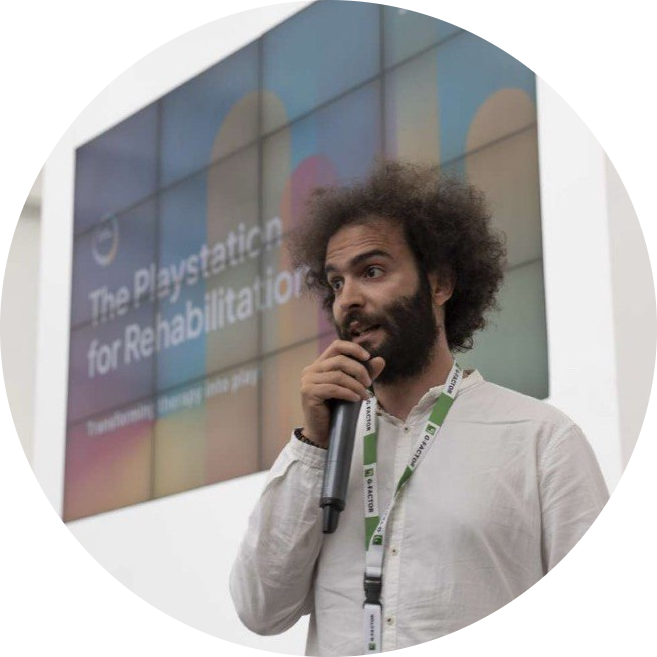
\includegraphics[width=2.8cm]{Pictures/Giovanni_pitch}
\end{minipage}
\vspace{0.1em}
}

\makeatletter
% the sender details are already in \clheader, so skip moderncv's own block
\@detailsfalse
% closing phrase, signature, name
\renewcommand*{\makeletterclosing}{%
  \@closing\\[0.6em]%
  
\includegraphics[height=1.2cm]{Pictures/sign_gt.jpg}\\[0.2em]%
  {\bfseries\@firstname~\@lastname}}
\makeatother


\begin{document}

\clheader{Product Designer \& Design Engineer | UX for Complex Systems}

\recipient{Product Design Hiring Team}{Revolut}
\opening{Dear Hiring Team,}
\closing{Yours faithfully,}
\makelettertitle

I am applying for the Platform Product Designer role. I am a designer and engineer (MSc in Design \& Engineering, Politecnico di Milano) with more than five years designing complex systems for expert users, at CNR-STIIMA, the Italian National Research Council, and as Head of Product and co-founder of Rehabilia Technologies.

The users I design for are operational ones: therapists and researchers who rely on a tool to get their daily work done. I designed the interface of PhiCube, a rehabilitation device, together with Italian clinics, to simplify how therapists configure hardware and software; it reached a usability score of 85.8/100 (SUS) with 19 children and is now in two ongoing multicentre studies with 134 patients.

I am comfortable with dense data and edge cases. For my PhD project, OmniTrack, I designed and built OmniAnalytics, a web dashboard for researchers with session browsing, synchronised time-series charts, trajectory playback and comparison tables. Much of the design work was in the exceptions: flows to correct missing or wrong sensor data, to exclude a trial or to relabel a session, without ever altering the raw records.

I think in systems and I can code. For OmniTrack I mapped the states, feedback logic and interactions across several devices, and I prototype in React and Python, so I understand backend-driven workflows and can test an idea with engineers early.

My process goes from research to flows, prototypes and usability tests, and as Head of Product I own it end to end, setting priorities with engineering and clinical teams. My products so far serve healthcare and research rather than finance, and at a smaller scale than Revolut's; the problems of fragmented workflows and demanding operational users are the ones I know. Examples of this work are in the portfolio linked above.

I would welcome the chance to discuss the role further.

\makeletterclosing

\end{document}
